\documentclass[conference]{IEEEtran}
\usepackage{cite}
\usepackage{amsmath}
\usepackage{graphicx}
\usepackage{booktabs}
\usepackage{multirow}
\usepackage{array}
\usepackage{microtype}
\usepackage{algorithm}
\usepackage[noend]{algpseudocode}
\PassOptionsToPackage{hyphens}{url}
\usepackage[hidelinks,breaklinks=true]{hyperref}
\usepackage{xurl}
\usepackage{xcolor}

% allow extra stretch in bibliography to prevent overfull hboxes
% caused by long URLs colliding with column boundaries
\setlength{\emergencystretch}{3em}

% float spacing tuned to avoid caption/text collisions in two-column layout
\setlength{\textfloatsep}{8pt plus 2pt minus 2pt}
\setlength{\dbltextfloatsep}{8pt plus 2pt minus 2pt}
\setlength{\floatsep}{6pt plus 2pt minus 2pt}
\setlength{\intextsep}{6pt plus 2pt minus 2pt}

\title{One Call, Two Outputs: Multilingual Voice-Based Injury Reporting and Surveillance in Ghana}

\author{%
  \IEEEauthorblockN{Yaw Osei Adjei,
                    Davis Opoku,
                    Kwadwo Amanqua Owusu, and
                    Benjamin Tei Partey}
  \IEEEauthorblockA{%
    Department of Computer Science\\
    Kwame Nkrumah University of Science and Technology\\
    Kumasi, Ghana\\
    yoadjei@st.knust.edu.gh,\;
    dopoku94@st.knust.edu.gh,\\
    kamanquaowusu@st.knust.edu.gh,\;
    parteybenjamintei@knust.edu.gh}%
}

\begin{document}

\maketitle

\begin{abstract}
Ghana recorded 2{,}949 road traffic deaths and 16{,}714 traffic injuries
in 2025, the highest annual fatality figure in 35
years~\cite{graphic2026_nrsa}. Few of these incidents are captured by
any health-information system, and existing emergency hotlines and
surveillance forms operate in English, which is a first language for
approximately 5\% of the population~\cite{ghc2021}.

This paper presents \textbf{VoiceTrace}, a five-stage natural language
processing (NLP) pipeline that accepts a spoken injury report in any
of five Ghanaian languages and returns two outputs from the same call:
a spoken first-aid response in the caller's language and a
structured, geocoded record for health surveillance. The pipeline
operates over a basic phone call and requires no English literacy or
smartphone hardware.

Evaluation uses 126 epidemiologically grounded synthetic injury
reports across five languages (Twi, Ga, Ewe, Fante, and Dagbani),
which together cover the first languages of approximately 85\% of
Ghana's population~\cite{ghc2021}. Three evaluation tracks isolate
distinct pipeline stages: end-to-end automatic speech recognition
(ASR) accuracy (Track~1); translation round-trip fidelity and
extraction $F_{1}$ on clean text (Track~2); and cross-language
extraction consistency (Track~3). Outcomes stratify by language. Twi
attains macro-$F_{1} = 0.66$ with Cohen's $\kappa = 0.80$ on clean
translated text, and macro-$F_{1} = 0.43$ after ASR at a word error
rate (WER) of 51.4\%. Fante attains macro-$F_{1} = 0.55$ with
$\kappa = 0.52$ on clean text, falling to macro-$F_{1} = 0.34$ after
ASR (WER 61.0\%). Ga, Ewe, and Dagbani record $\kappa < 0.13$,
mirroring lower BLEU and BERTScore values for those languages and
indicating that the binding constraint is the available
machine-translation (MT) capacity rather than the extraction
architecture.

The system constitutes the first reported end-to-end voice pipeline
for injury management and surveillance in any Ghanaian language.
\end{abstract}

\begin{IEEEkeywords}
injury surveillance, multilingual NLP, African languages, automatic
speech recognition, large language models, Ghana, voice-first
systems, emergency response, low-resource NLP
\end{IEEEkeywords}


%% =========================================================
\section{Introduction}
%% =========================================================

The conference theme, \textit{Harnessing Evidence from Local Research
to Address the Rising Challenges of Injury Management}, requires
locally generated evidence directed at injury management as well as
prevention. The work reported here addresses both requirements
through a system designed for community-scale operation in Ghana.

In high-income settings, an emergency call typically performs two
functions concurrently: response dispatch to the caller and the
creation of a structured record for public health surveillance. In
Ghana, neither function is currently available at community scale in
local languages.

The injury burden is measurable and increasing. Ghana recorded
2{,}949 road traffic deaths in 2025, the highest annual figure in
35 years, with a further 16{,}714 people injured in the same crashes
\cite{graphic2026_nrsa}. The Global Burden of Disease 2021 study
ranks injuries among the top five contributors to years of life lost
in Ghana~\cite{ihme_gbd}. Road traffic accidents (RTAs) accounted for
39\% of injury presentations at Korle-Bu Teaching
Hospital~\cite{boateng2019}, and the demographic concentration of
injury falls on males aged 15--34 \cite{dhs2008,dhs2022}. Surveillance
coverage is weakest in the rural and peri-urban communities where
crash density is highest and facility access is
slowest~\cite{mesic2024}.

The principal limitation is linguistic access. English is a first
language for approximately 5\% of Ghanaians, while every existing
health hotline and surveillance form operates in English. According
to the 2021 Population and Housing Census, Akan languages (Twi and
Fante) are spoken by 45--47\% of the population, Ewe by 13--14\%,
Ga-Dangme by 7\%, and the Mole-Dagbani cluster by 18--19\%
\cite{ghc2021}. The five languages evaluated in this paper jointly
cover approximately 85\% of first-language speakers, distributed
across regions as shown in Fig.~\ref{fig:lang_map}.

\begin{figure}[!t]
\centering
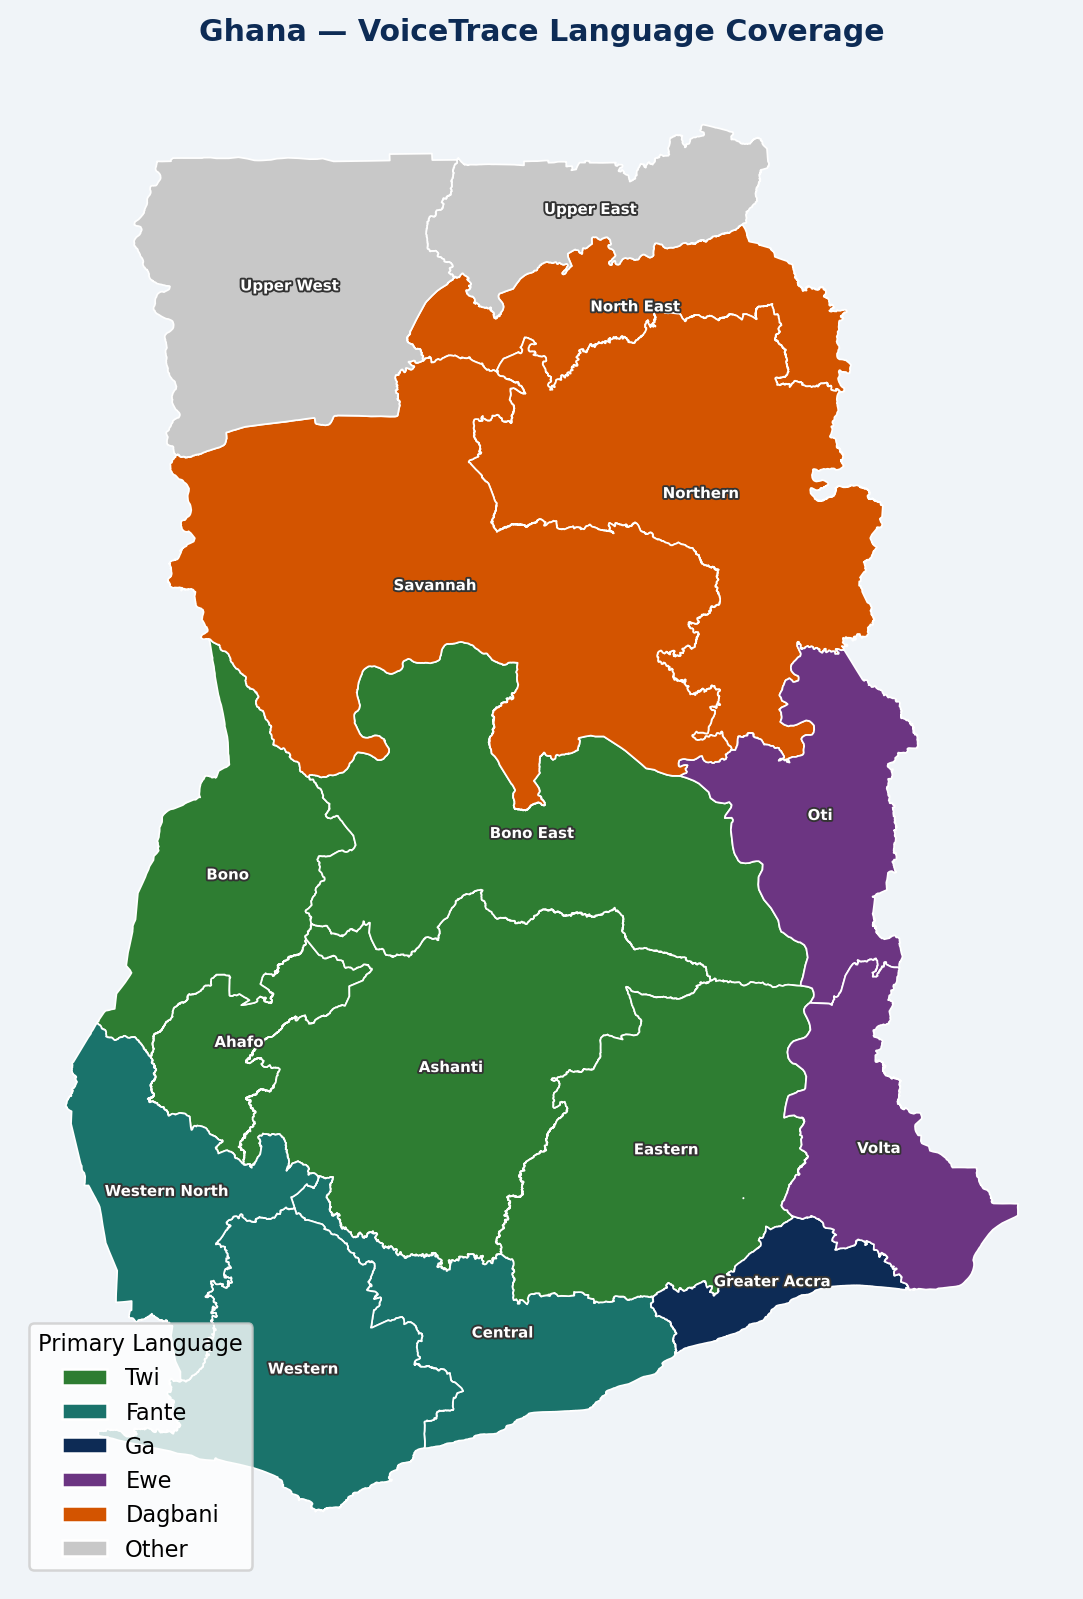
\includegraphics[width=0.92\columnwidth]{figures/ghana_language_map.png}
\caption{Regional distribution of the five evaluated primary languages
in Ghana, drawn from~\cite{ghc2021}.}
\label{fig:lang_map}
\end{figure}

The component technologies required to address the gap are already
available within Ghana. The GhanaNLP consortium provides
Khaya~\cite{khaya}, an integrated platform that supports automatic
speech recognition (ASR), neural machine translation (MT), and
text-to-speech (TTS) across nine Ghanaian languages. Recent work on
zero-shot extraction with large language models (LLMs) reports
performance comparable to that of fine-tuned models in data-scarce
clinical domains~\cite{omiye2025,lorenzoni2024}. Until this work,
these capabilities have not been integrated into an end-to-end
pipeline targeted at injury response and surveillance.

\textbf{Contributions.} This paper makes three contributions:
\begin{enumerate}
  \item \textbf{System.} \textbf{VoiceTrace}, a five-stage voice
  pipeline that accepts a spoken injury report in any of five
  Ghanaian languages and produces, from the same call, a spoken
  first-aid response to the caller and a structured geocoded record
  for surveillance.
  \item \textbf{Corpus.} An epidemiologically grounded synthetic
  evaluation corpus of 126 injury narratives, sampled from
  Ghana-specific distributions and rendered in five Ghanaian
  languages through Khaya MT and TTS.
  \item \textbf{Evaluation.} A three-track quantitative analysis that
  separates ASR error, translation fidelity, and extraction
  consistency, and identifies the binding constraint per language.
\end{enumerate}

VoiceTrace is designed to function as the NLP core of a deployable
community emergency line, accessible through a dedicated shortcode,
with surveillance records forwarded to the District Health
Information Management System (DHIMS-2) and emergency notifications
routed to the National Ambulance Service dispatch network. The
present paper evaluates the pipeline in isolation; deployment
infrastructure is treated as future work.

The pipeline produces two outputs from a single call. The
caller-facing output supports injury management in the pre-facility
window: ASR transcribes the report, MT renders it in English,
extraction by Claude (\texttt{claude-sonnet-4-6}) selects structured
fields and generates a brief first-aid message, geocoding identifies
the nearest Ghana Health Service facility, and TTS returns the
response in the caller's language. The system-facing output supports
surveillance: the same extraction step yields a structured record
against a six-field schema, augmented with geocoded coordinates and
a facility recommendation, and written to the surveillance log
without a separate reporting action.

No labelled speech corpus for injury reporting was available in any
Ghanaian language at the time of this work. The evaluation corpus is
therefore synthetic: 126 English narratives sampled to match
published Ghanaian injury distributions
\cite{boateng2019,opoku2025,mesic2024}, translated into five target
languages via Khaya MT, and synthesised to audio via Khaya TTS.

The remainder of the paper is organised as follows.
Section~\ref{sec:related} situates the work in related literature.
Section~\ref{sec:data} describes corpus construction.
Section~\ref{sec:arch} details the pipeline architecture.
Section~\ref{sec:eval} reports the evaluation framework and results.
Section~\ref{sec:discussion} addresses limitations, clinical safety,
and the deployment pathway. Section~\ref{sec:conclusion} concludes.


%% =========================================================
\section{Related Work}
\label{sec:related}
%% =========================================================

\subsection{Injury Surveillance in Low- and Middle-Income Countries}
Vallmuur~\cite{vallmuur2015} established that NLP can systematically
code injury cause from unstructured emergency-department text in
English, providing the methodological foundation for automated
extraction from injury narratives. The present work extends that
foundation to spoken community reports in low-resource African
languages. Mesic et al.~\cite{mesic2024} demonstrated that
computational hotspot analysis of road crashes in Greater Accra is
feasible from non-clinical data, supporting the use of geocoded
location fields for spatial surveillance. The geocoding stage in
Section~\ref{sec:arch} builds on this finding.

\subsection{Speech Recognition for African Languages}
The Khaya platform~\cite{khaya} supplies ASR, MT, and TTS for nine
Ghanaian languages and is the most capable openly available system
for this language family. General-purpose multilingual models such as
Whisper~\cite{radford2023} exhibit reduced accuracy on African
languages with limited training representation. Khaya is used
throughout the pipeline because it provides the full
ASR$\rightarrow$MT$\rightarrow$TTS loop required for closed-loop
interaction in the target languages.

\subsection{LLM-Based Clinical Information Extraction}
Omiye et al.~\cite{omiye2025} and Lorenzoni et al.~\cite{lorenzoni2024}
report that zero-shot LLM extraction with structured prompts attains
performance comparable to fine-tuned models in data-scarce clinical
domains. The present work adopts this approach because no
Ghanaian-language training data exists for a fine-tuned alternative.

\subsection{Synthetic Corpora for Low-Resource NLP}
Nyamawe and Shao~\cite{nyamawe2026} introduced the use of
LLM-generated synthetic evaluation corpora for low-resource African
NLP. The present work extends that methodology with an
epidemiological grounding step: narratives are sampled from the
empirical distributions reported in \cite{boateng2019,opoku2025},
producing a corpus that reflects the documented Ghanaian injury
burden rather than unconstrained generation.

\subsection{Voice-Based Health Systems in Low-Resource Settings}
Interactive voice response (IVR) systems deployed for health
information in low- and middle-income countries follow fixed
decision trees and do not accept open-ended natural language
input~\cite{who_ghe}. VoiceTrace processes unstructured free-form
speech and produces contextually adaptive responses through an LLM.
No prior system has reported this capability for Ghanaian languages
in a health context.


%% =========================================================
\section{Dataset Construction}
\label{sec:data}
%% =========================================================

\subsection{Motivation}
A targeted literature review identified no labelled dataset of spoken
injury reports in any Ghanaian language. Published speech corpora for
these languages cover general domains and do not include injury or
emergency content. Real caller data was not collected at the
prototype stage for two reasons: informed consent from distressed
callers is operationally difficult, and a labelled corpus of
sufficient size would itself require deployment. The evaluation
corpus is therefore synthetic, sampled from published Ghanaian
injury distributions to remain reproducible and externally grounded.

\subsection{Epidemiological Grounding}
The corpus comprises 126 English-language injury narratives sampled
across six fields (Table~\ref{tab:distributions}). Injury-type
proportions are taken from Boateng et al.~\cite{boateng2019}
($n = 1{,}238$, Korle-Bu Teaching Hospital). Severity and pooled
prevalence follow Opoku et al.~\cite{opoku2025}. Age and sex
distributions follow the Demographic and Health Survey (DHS) injury
modules of 2008 and 2022~\cite{dhs2008,dhs2022}. Location-type
proportions follow Mesic et al.~\cite{mesic2024}. Aggregate burden
framing draws on the Global Burden of Disease (GBD)~\cite{ihme_gbd}
and the World Health Organization Global Health Estimates
(GHE)~\cite{who_ghe}.

\begin{table}[!t]
\caption{Synthetic narrative sampling distributions.}
\label{tab:distributions}
\centering
\begin{tabular}{ll}
\toprule
\textbf{Field} & \textbf{Distribution} \\
\midrule
Injury type   & RTA 39.1\%, Fall 19.7\%, Assault 12.0\%, \\
              & Burn 8.5\%, Drowning 4.3\%, Occupational 16.4\% \\
Sex           & Male 67.8\%, Female 32.2\% \\
Age group     & $<$15: 18\%, 15--34: 45\%, 35--54: 27\%, 55+: 10\% \\
Severity      & Minor 52\%, Moderate 31\%, Severe 17\% \\
Body region   & Head/neck 38\%, Limb 44\%, Trunk 18\% \\
Location type & Highway 41\%, Urban road 35\%, Home 24\% \\
\bottomrule
\end{tabular}
\end{table}

\subsection{Narrative Generation and Synthesis}
Narratives were produced with Claude
(\texttt{claude-sonnet-4-6})~\cite{anthropic2024}, conditioned on
per-language persona prompts that encode regional dialect, register,
and community context. Prompts were reviewed for cultural
plausibility by the first author, a native Ghanaian. The English
narratives were translated into Twi, Ga, Ewe, Fante, and Dagbani
through Khaya MT, then converted to audio with Khaya TTS v2
(IEEE-float WAV). Inputs longer than the 450-character API limit
were segmented at sentence boundaries; the resulting audio segments
were concatenated. A normalisation step collapsed pathological
diacritic repetition (e.g., \textit{ɛɛ}$\rightarrow$\textit{ɛ},
\textit{ɔɔ}$\rightarrow$\textit{ɔ}), which had triggered TTS looping
artefacts. Normalisation was applied only at synthesis time; source
text was preserved for evaluation.

\subsection{Gold Annotation}
The 126 English narratives were annotated against the six-field
schema in Table~\ref{tab:schema} using a two-pass single-annotator
protocol with a minimum inter-pass interval of 24 hours.
Inter-pass disagreements were reconciled by deliberation to yield a
single gold standard, which serves as the reference across the three
evaluation tracks. The two-pass procedure yields an inter-pass
agreement statistic that serves as a proxy for inter-annotator
reliability; multi-annotator labelling is identified as a priority
for any subsequent corpus release (Section~\ref{sec:limitations}).

\begin{table}[!t]
\caption{Gold-annotation schema.}
\label{tab:schema}
\centering
\small
\begin{tabular}{ll}
\toprule
\textbf{Field} & \textbf{Values} \\
\midrule
\texttt{injury\_type}          & rta, fall, assault, burn, drowning, \\
                               & occupational, unknown \\
\texttt{severity}              & minor, moderate, severe, unknown \\
\texttt{body\_region}          & head\_neck, upper\_limb, lower\_limb, \\
                               & trunk, multiple, unknown \\
\texttt{victim\_sex}           & male, female, unknown \\
\texttt{victim\_age\_group}    & child, youth, adult, elderly, unknown \\
\texttt{location\_description} & free text ($\leq$15 words) \\
\bottomrule
\end{tabular}
\end{table}

A free-text \texttt{mechanism} field is also produced by the
extraction step and retained in pipeline output, but is excluded from
the categorical $F_{1}$ evaluation reported in
Section~\ref{sec:eval}.


%% =========================================================
\section{System Architecture}
\label{sec:arch}
%% =========================================================

The pipeline comprises five sequential stages and produces two
outputs from a single call: a spoken response to the caller and a
structured surveillance record (Fig.~\ref{fig:architecture}).

\begin{figure}[!t]
\centering
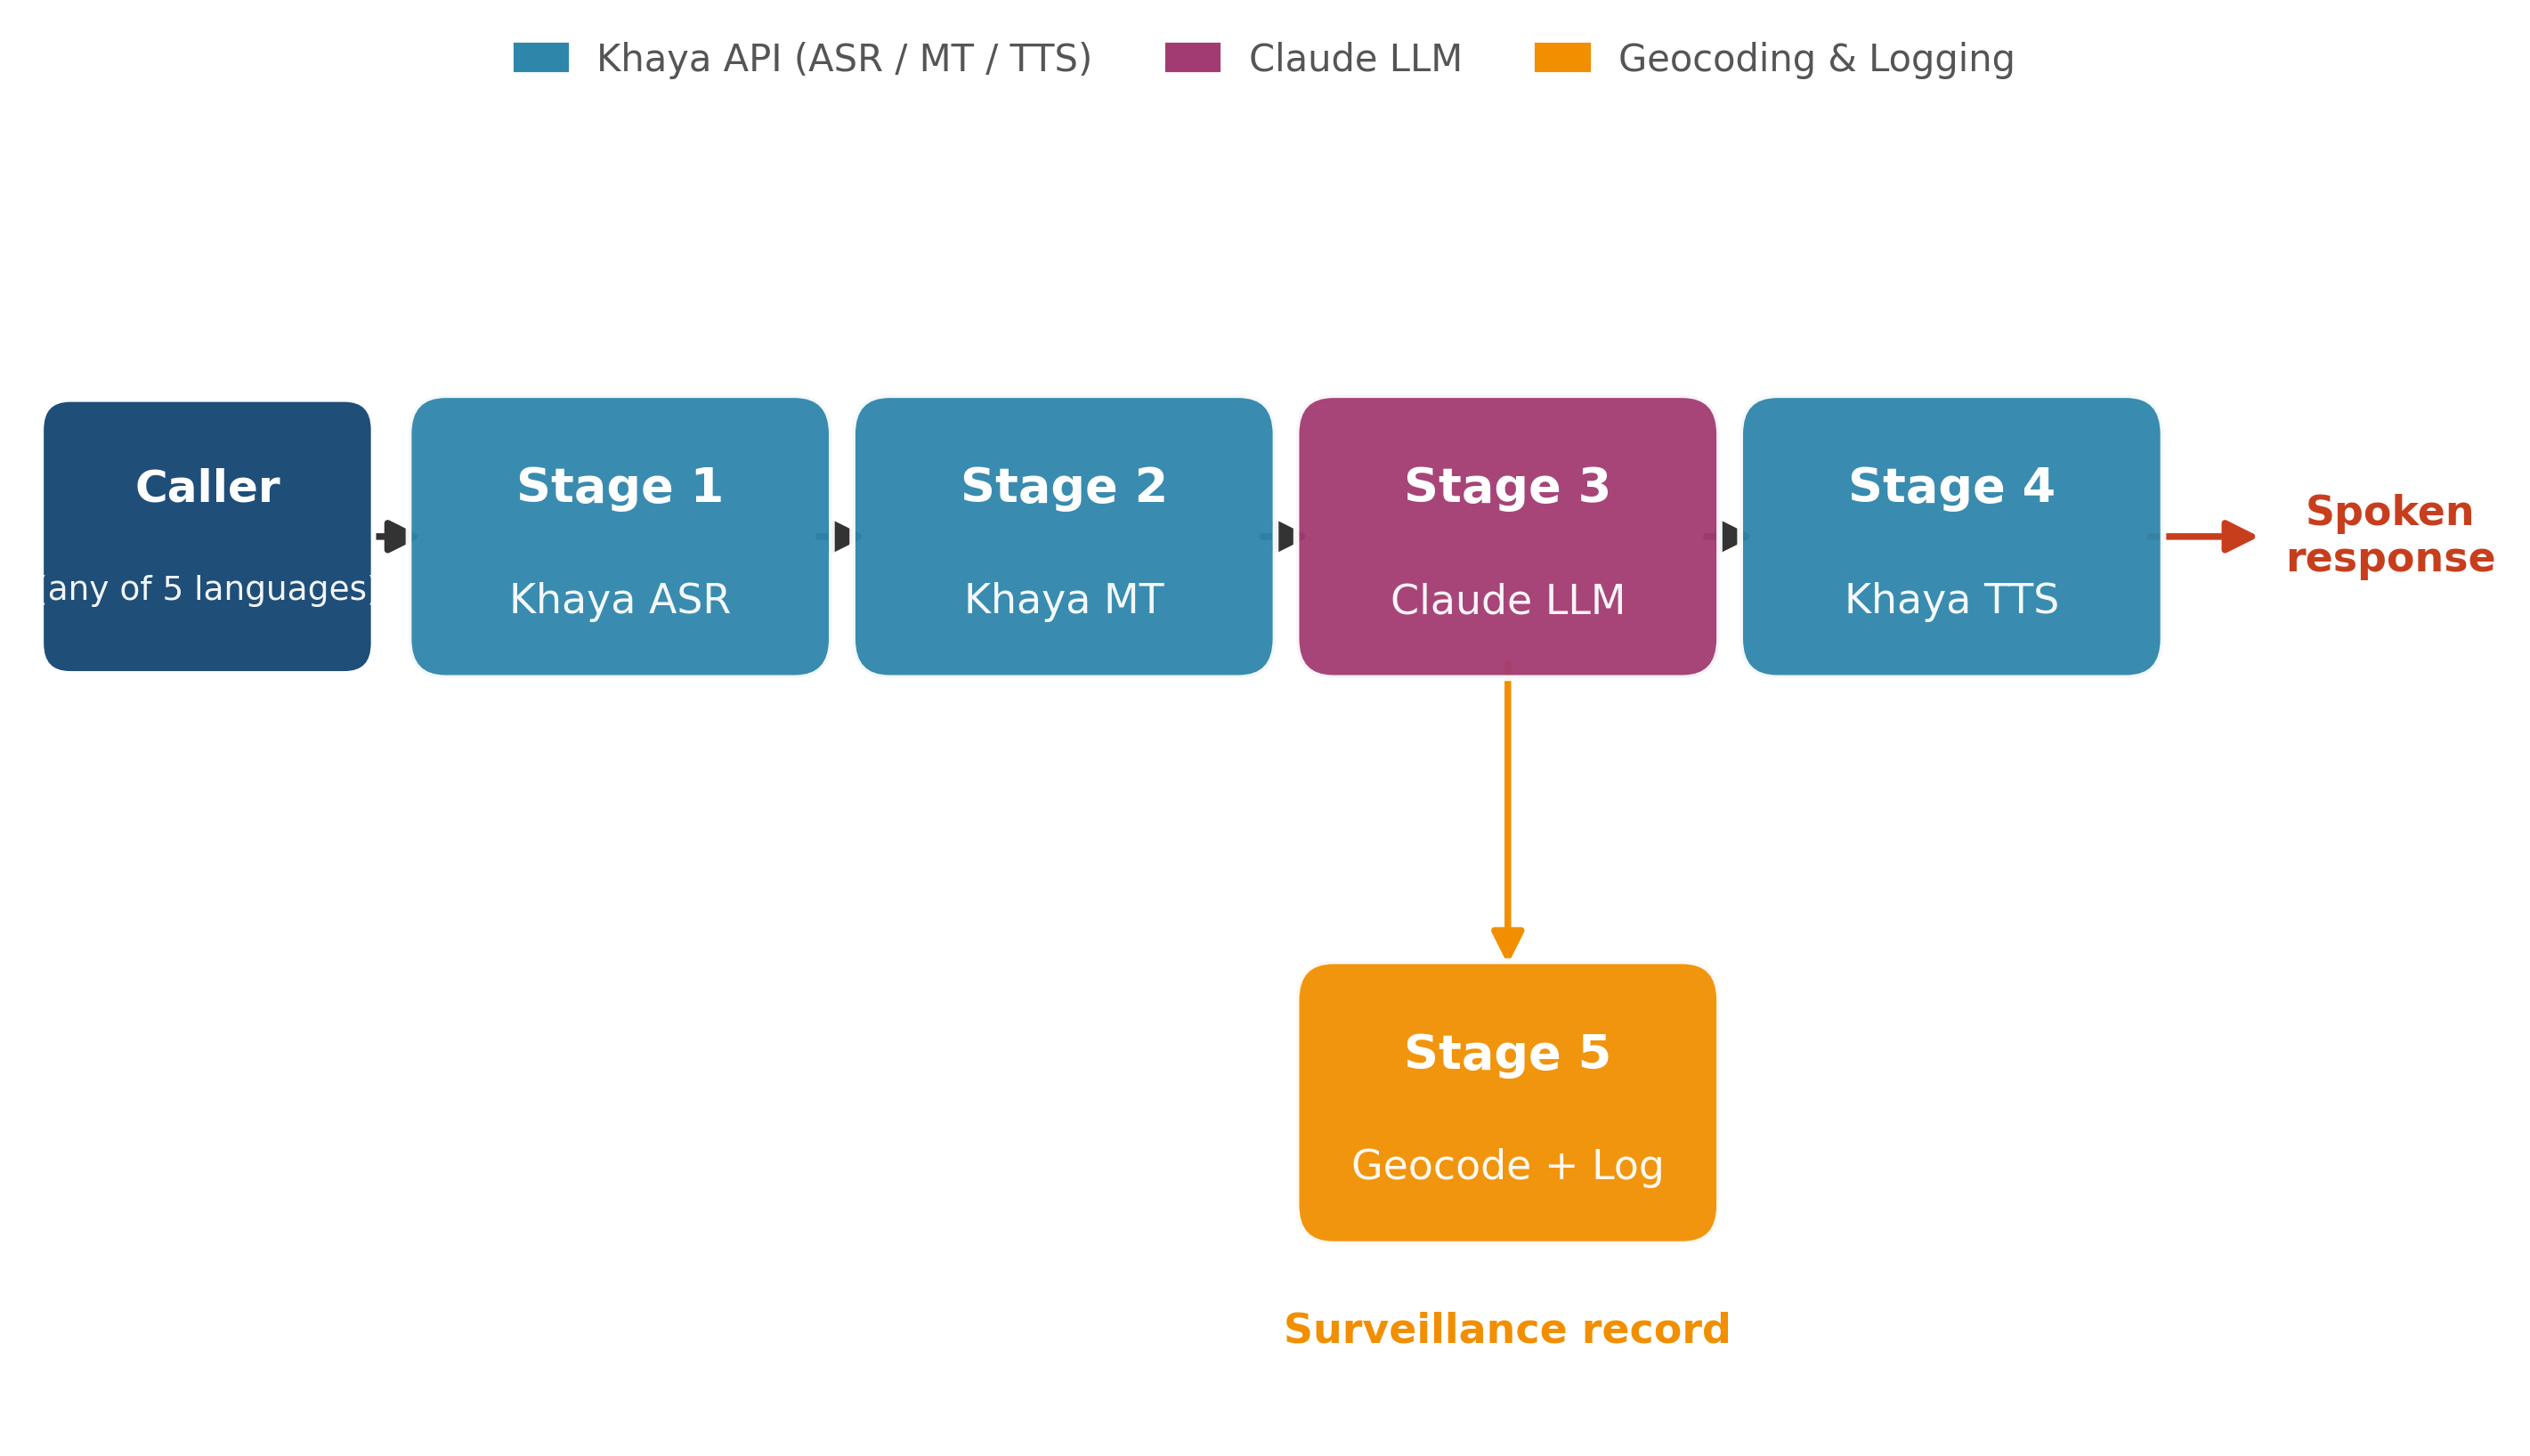
\includegraphics[width=\columnwidth]{figures/architecture_diagram.png}
\caption{Five-stage VoiceTrace pipeline. Stages~1--4 serve the caller
in real time; Stage~5 produces a structured surveillance record in
parallel.}
\label{fig:architecture}
\end{figure}

\subsection{Stage 1: Automatic Speech Recognition}
Caller audio is submitted to the Khaya ASR endpoint
(\texttt{/asr/v3/transcribe}) together with the identified
language code; the service returns a Ghanaian-language transcript.
A failed request returns an empty string, which downstream stages
propagate as an \texttt{unknown} record without interrupting the
call.

\subsection{Stage 2: Machine Translation}
The Ghanaian-language transcript is translated to English through
Khaya MT. The intermediate English representation enables a single
language-agnostic extraction prompt to serve all five target
languages, removing the need for language-specific extraction models.

\subsection{Stage 3: Extraction and First-Aid Generation}
The English translation is passed to Claude
(\texttt{claude-sonnet-4-6})~\cite{anthropic2024} under a single
zero-shot prompt that returns two outputs.

\textbf{(a) Structured extraction.} The six annotation fields in
Table~\ref{tab:schema} are returned as JSON. Fields that the input
underdetermines are encoded as \texttt{"unknown"}. Invalid JSON
responses are logged and converted to a record in which all fields
are \texttt{"unknown"}.

\textbf{(b) First-aid generation.} A brief spoken first-aid message
is produced from the extracted injury type, severity, and body
region. Every response ends with a mandatory closing instruction
that directs the caller to the nearest health facility. The system
prompt prohibits diagnostic claims, drug recommendations, and
treatment specifications (Section~\ref{sec:safety}).

Algorithm~\ref{alg:stage3} summarises the Stage-3 procedure with
the relevant decoding and safety parameters fixed.

\begin{algorithm}[!t]
\caption{Stage-3 extraction and first-aid generation.}
\label{alg:stage3}
\begin{algorithmic}[1]
\Require English transcript $x$, schema $\mathcal{S}$, system
prompt $P_{\mathrm{sys}}$, model $M$
\Ensure structured record $r$, first-aid text $a$
\State $P \gets P_{\mathrm{sys}} \,\Vert\, \mathcal{S} \,\Vert\, x$
\Comment{single zero-shot prompt}
\State $y \gets M(P;\, T = 0.2,\, \text{max\_tokens} = 800)$
\State $\{r, a\} \gets \textsc{ParseJSON}(y)$
\If{$\textsc{ParseJSON}$ fails \textbf{or}
    $r \not\models \mathcal{S}$}
  \State $r \gets \{f \mapsto \texttt{"unknown"} :
                    f \in \mathcal{S}\}$
  \State \textsc{LogParseFailure}$(y)$
\EndIf
\State $a \gets \textsc{EnforceSafetyClosing}(a)$
\Comment{appends facility-referral sentence}
\State \Return $r$, $a$
\end{algorithmic}
\end{algorithm}

The decoding temperature $T = 0.2$ is selected to suppress lexical
variation in clinical phrasing while retaining enough flexibility for
fluent prose. The schema $\mathcal{S}$ is the field--value mapping
of Table~\ref{tab:schema}; $r \models \mathcal{S}$ requires every
field to take a value from its declared vocabulary.
\textsc{EnforceSafetyClosing} appends the standard facility-referral
sentence when the generated text omits it.

\subsection{Stage 4: Text-to-Speech}
The first-aid text is translated from English to the caller's
language through Khaya MT and synthesised with Khaya TTS v2. The
caller receives the response as audio in the same language used
during the call.

\subsection{Stage 5: Geocoding and Surveillance Logging}
The \texttt{location\_description} from Stage~3 is geocoded through
Nominatim/OpenStreetMap with the search bounded to Ghana. The
resolved coordinates are matched to the nearest facility in the
Ghana Health Service registry. The structured record, the facility
recommendation, and the coordinates are appended to the surveillance
log as a single row, generated as a byproduct of the caller
interaction.


%% =========================================================
\section{Evaluation}
\label{sec:eval}
%% =========================================================

The evaluation is structured as three tracks. Each track isolates a
distinct pipeline component and addresses a separate question about
deployment readiness or language equity.

\subsection{Track 1: Full Pipeline (Twi and Fante)}

Track~1 exercises the complete pipeline. TTS-synthesised audio is
processed through Khaya ASR, translated to English through Khaya MT,
and passed to Claude for extraction.

ASR performance is reported as Word Error Rate
(WER)~\cite{morris2004}, computed with \texttt{jiwer} between Khaya
ASR output and the source transcript. WER is reported overall and by
injury type. Because the audio used for evaluation is itself
TTS-synthesised, the reported WER provides a lower bound on the WER
expected from natural community speech.

Per-field precision, recall, and $F_{1}$ are computed with
\texttt{sklearn.metrics.classification\_report}. The headline metric
is macro-averaged $F_{1}$ over the five categorical fields. The
delta between Track~1 (post-ASR) macro-$F_{1}$ and Track~2 (clean
text) macro-$F_{1}$ quantifies the accuracy loss attributable to the
ASR stage.

\subsection{Track 2: Translation Round-Trip and Extraction (Five Languages)}

Track~2 measures the information that survives translation before
extraction is attempted. Each English narrative is translated to a
target language through Khaya MT, then translated back to English.
Round-trip fidelity is measured with BERTScore
$F_{1}$~\cite{zhang2019bertscore} and BLEU computed by
\texttt{sacrebleu}, both against the original English. Claude
extraction is then run on the round-tripped English, and $F_{1}$ is
computed against the gold annotations.

\subsection{Track 3: Cross-Language Extraction Consistency (Five Languages)}

Track~3 measures whether the pipeline produces consistent
surveillance classifications across input languages for the same
underlying scenario. Cohen's $\kappa$ is computed across language
pairs and per extraction field with
\texttt{sklearn.metrics.cohen\_kappa\_score}. High pairwise $\kappa$
indicates equitable output: the same scenario yields the same record
regardless of input language.

\subsection{Results}

The five evaluated languages stratify into two performance bands.
Twi and Fante constitute Tier~1: extraction output agrees
substantially with expert annotation, and the pipeline produces
usable surveillance records. Ga, Ewe, and Dagbani constitute
Tier~2: extraction agreement against gold sits near the
chance-agreement band. The discussion in
Section~\ref{sec:discussion} attributes the Tier-2 outcome to MT
fidelity rather than to extraction-architecture failure.

\paragraph{ASR results.}
Table~\ref{tab:wer_all} reports overall WER across the five
languages. Ga is an outlier at 80.9\%, exceeding the next-highest
language by 19.9~percentage points; the cause is examined in
Section~\ref{sec:ga_outlier}. Within Twi, WER varies modestly across
injury type (47.5\% to 53.2\%; Fig.~\ref{fig:wer},
Table~\ref{tab:wer}). Assault narratives are transcribed most
accurately, while RTA and fall narratives are transcribed least
accurately, consistent with the higher density of road, vehicle, and
body-region terms in the latter categories.

\begin{table}[!t]
\caption{ASR word error rate across five languages ($n = 80$ each).}
\label{tab:wer_all}
\centering
\begin{tabular}{lcc}
\toprule
\textbf{Language} & \textbf{Overall WER (\%)}
                  & \textbf{Range across injury types (\%)} \\
\midrule
Twi              & 51.4 & 47.5--53.2 \\
Fante            & 61.0 & 53.8--63.2 \\
Ewe              & 56.1 & 52.2--57.9 \\
Dagbani          & 54.1 & 47.7--56.1 \\
\textbf{Ga}      & \textbf{80.9} & \textbf{76.5--83.9} \\
\bottomrule
\end{tabular}
\end{table}

\begin{figure}[!t]
\centering
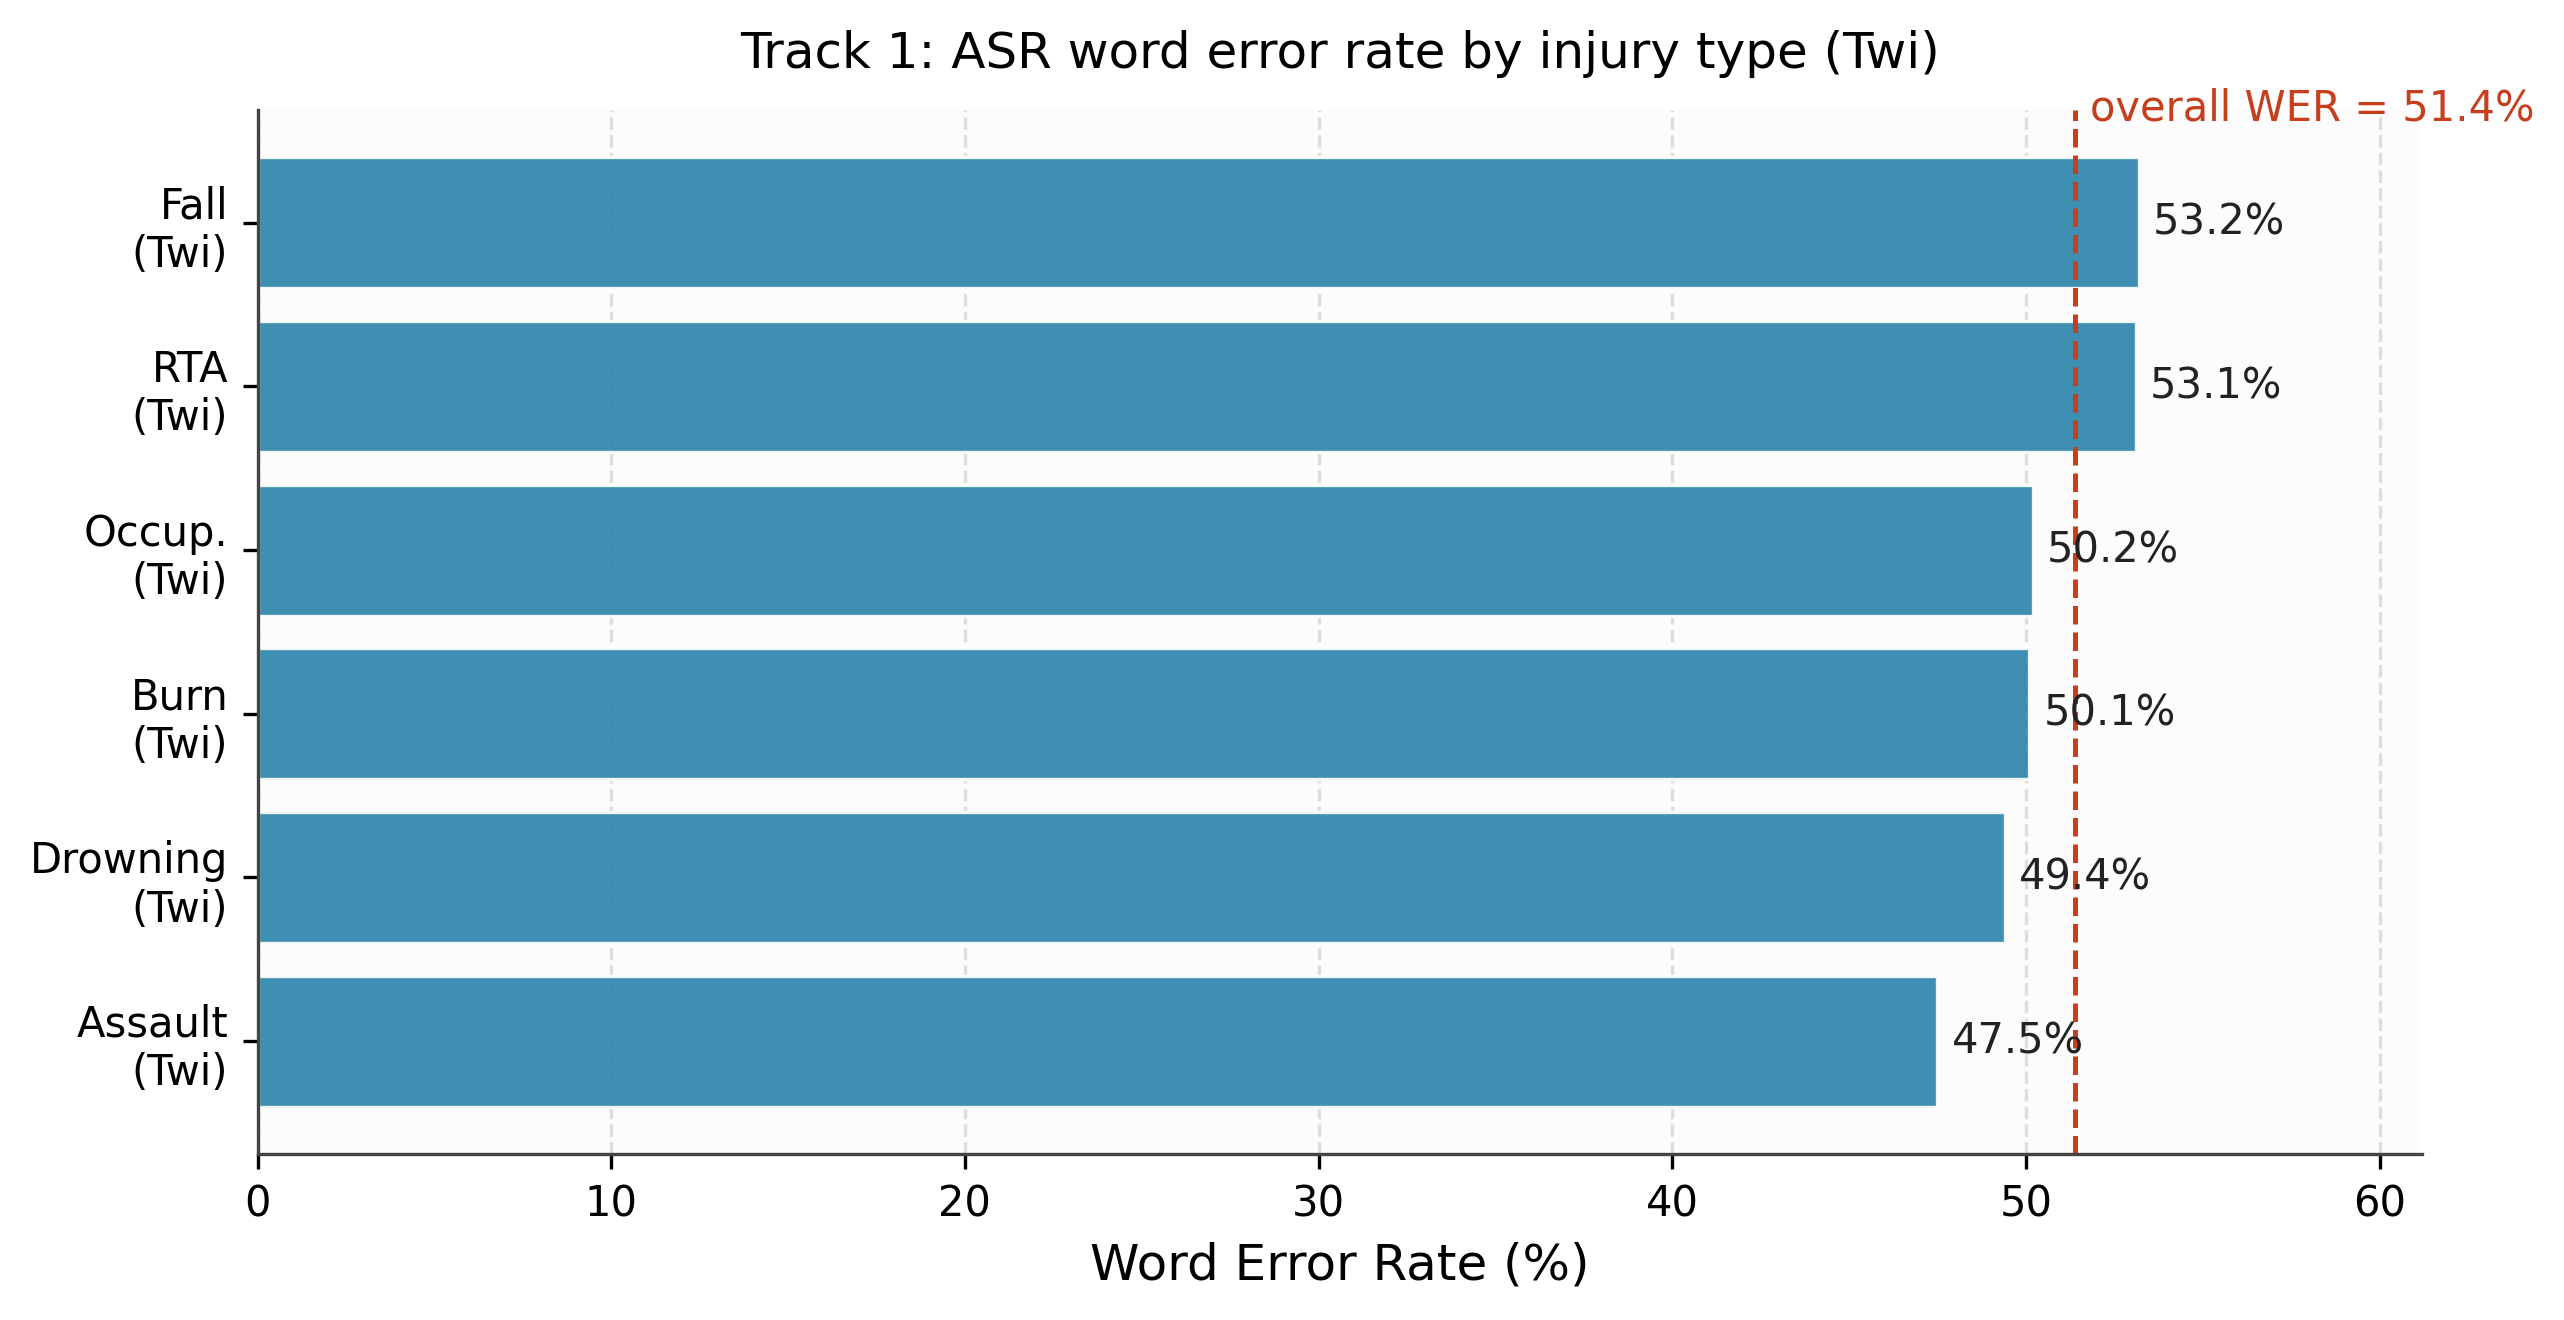
\includegraphics[width=\columnwidth]{figures/wer_by_injury.png}
\caption{Track~1 WER by injury type for Twi.}
\label{fig:wer}
\end{figure}

\begin{table}[!t]
\caption{Track~1 ASR performance by injury type (Twi, $n = 80$).}
\label{tab:wer}
\centering
\begin{tabular}{lc}
\toprule
\textbf{Injury Type} & \textbf{WER (\%)} \\
\midrule
Road traffic accident & 53.1 \\
Fall                  & 53.2 \\
Assault               & 47.5 \\
Burn                  & 50.1 \\
Drowning              & 49.4 \\
Occupational          & 50.2 \\
\midrule
\textbf{Overall}      & \textbf{51.4} \\
\bottomrule
\end{tabular}
\end{table}

\paragraph{Track-1 extraction.}
Table~\ref{tab:f1_t1} reports per-field $F_{1}$ after full ASR
transcription for the two Tier-1 languages. Twi macro-$F_{1}$ falls
from 0.66 on clean text to 0.43 after ASR ($\Delta = 0.23$). The
severity field shows the largest reduction ($F_{1} = 0.29$),
indicating that severity is conveyed through lexical features that
are sensitive to ASR substitution errors. Fante macro-$F_{1}$ falls
from 0.55 to 0.34 ($\Delta = 0.21$), consistent with the higher
baseline WER of 61.0\%.

\begin{table}[!t]
\caption{Track~1 extraction $F_{1}$ by field, Twi and Fante
(post-ASR).}
\label{tab:f1_t1}
\centering
\small
\setlength{\tabcolsep}{4pt}
\begin{tabular}{lcccc}
\toprule
\textbf{Field}
  & \multicolumn{2}{c}{\textbf{Twi (WER 51.4\%)}}
  & \multicolumn{2}{c}{\textbf{Fante (WER 61.0\%)}} \\
\cmidrule(lr){2-3}\cmidrule(lr){4-5}
  & $F_{1}$ & \textbf{P / R}
  & $F_{1}$ & \textbf{P / R} \\
\midrule
injury\_type       & 0.52 & 0.68 / 0.44 & 0.36 & 0.50 / 0.30 \\
severity           & 0.29 & 0.38 / 0.24 & 0.25 & 0.47 / 0.18 \\
body\_region       & 0.48 & 0.69 / 0.45 & 0.29 & 0.58 / 0.20 \\
victim\_sex        & 0.45 & 0.55 / 0.39 & 0.37 & 0.50 / 0.30 \\
victim\_age\_group & 0.43 & 0.49 / 0.49 & 0.40 & 0.49 / 0.51 \\
\midrule
\textbf{Macro avg} & \textbf{0.43} & & \textbf{0.34} & \\
\bottomrule
\end{tabular}
\end{table}

\paragraph{Track-2 fidelity and extraction.}
Table~\ref{tab:t2} reports BERTScore $F_{1}$, BLEU, and macro-$F_{1}$
on clean translated text. Twi records the lowest BERTScore (0.369)
and the highest extraction $F_{1}$ (0.66), an inversion that is
discussed in Section~\ref{sec:discussion}. Fante records the highest
BERTScore (0.695) and the second-highest extraction $F_{1}$ (0.55).
Figure~\ref{fig:f1_langs} visualises the three Track-2 metrics
side by side.

\begin{table}[!t]
\caption{Track~2 round-trip fidelity and extraction $F_{1}$
($n = 80$ per language).}
\label{tab:t2}
\centering
\begin{tabular}{lccc}
\toprule
\textbf{Language} & \textbf{BERTScore $F_{1}$}
                  & \textbf{BLEU}
                  & \textbf{Macro $F_{1}$} \\
\midrule
Twi     & 0.369 & 1.86  & 0.660 \\
Fante   & 0.695 & 15.86 & 0.553 \\
Ewe     & 0.571 & 6.55  & 0.233 \\
Ga      & 0.513 & 3.96  & 0.186 \\
Dagbani & 0.521 & 3.95  & 0.173 \\
\bottomrule
\end{tabular}
\end{table}

\begin{figure}[!t]
\centering
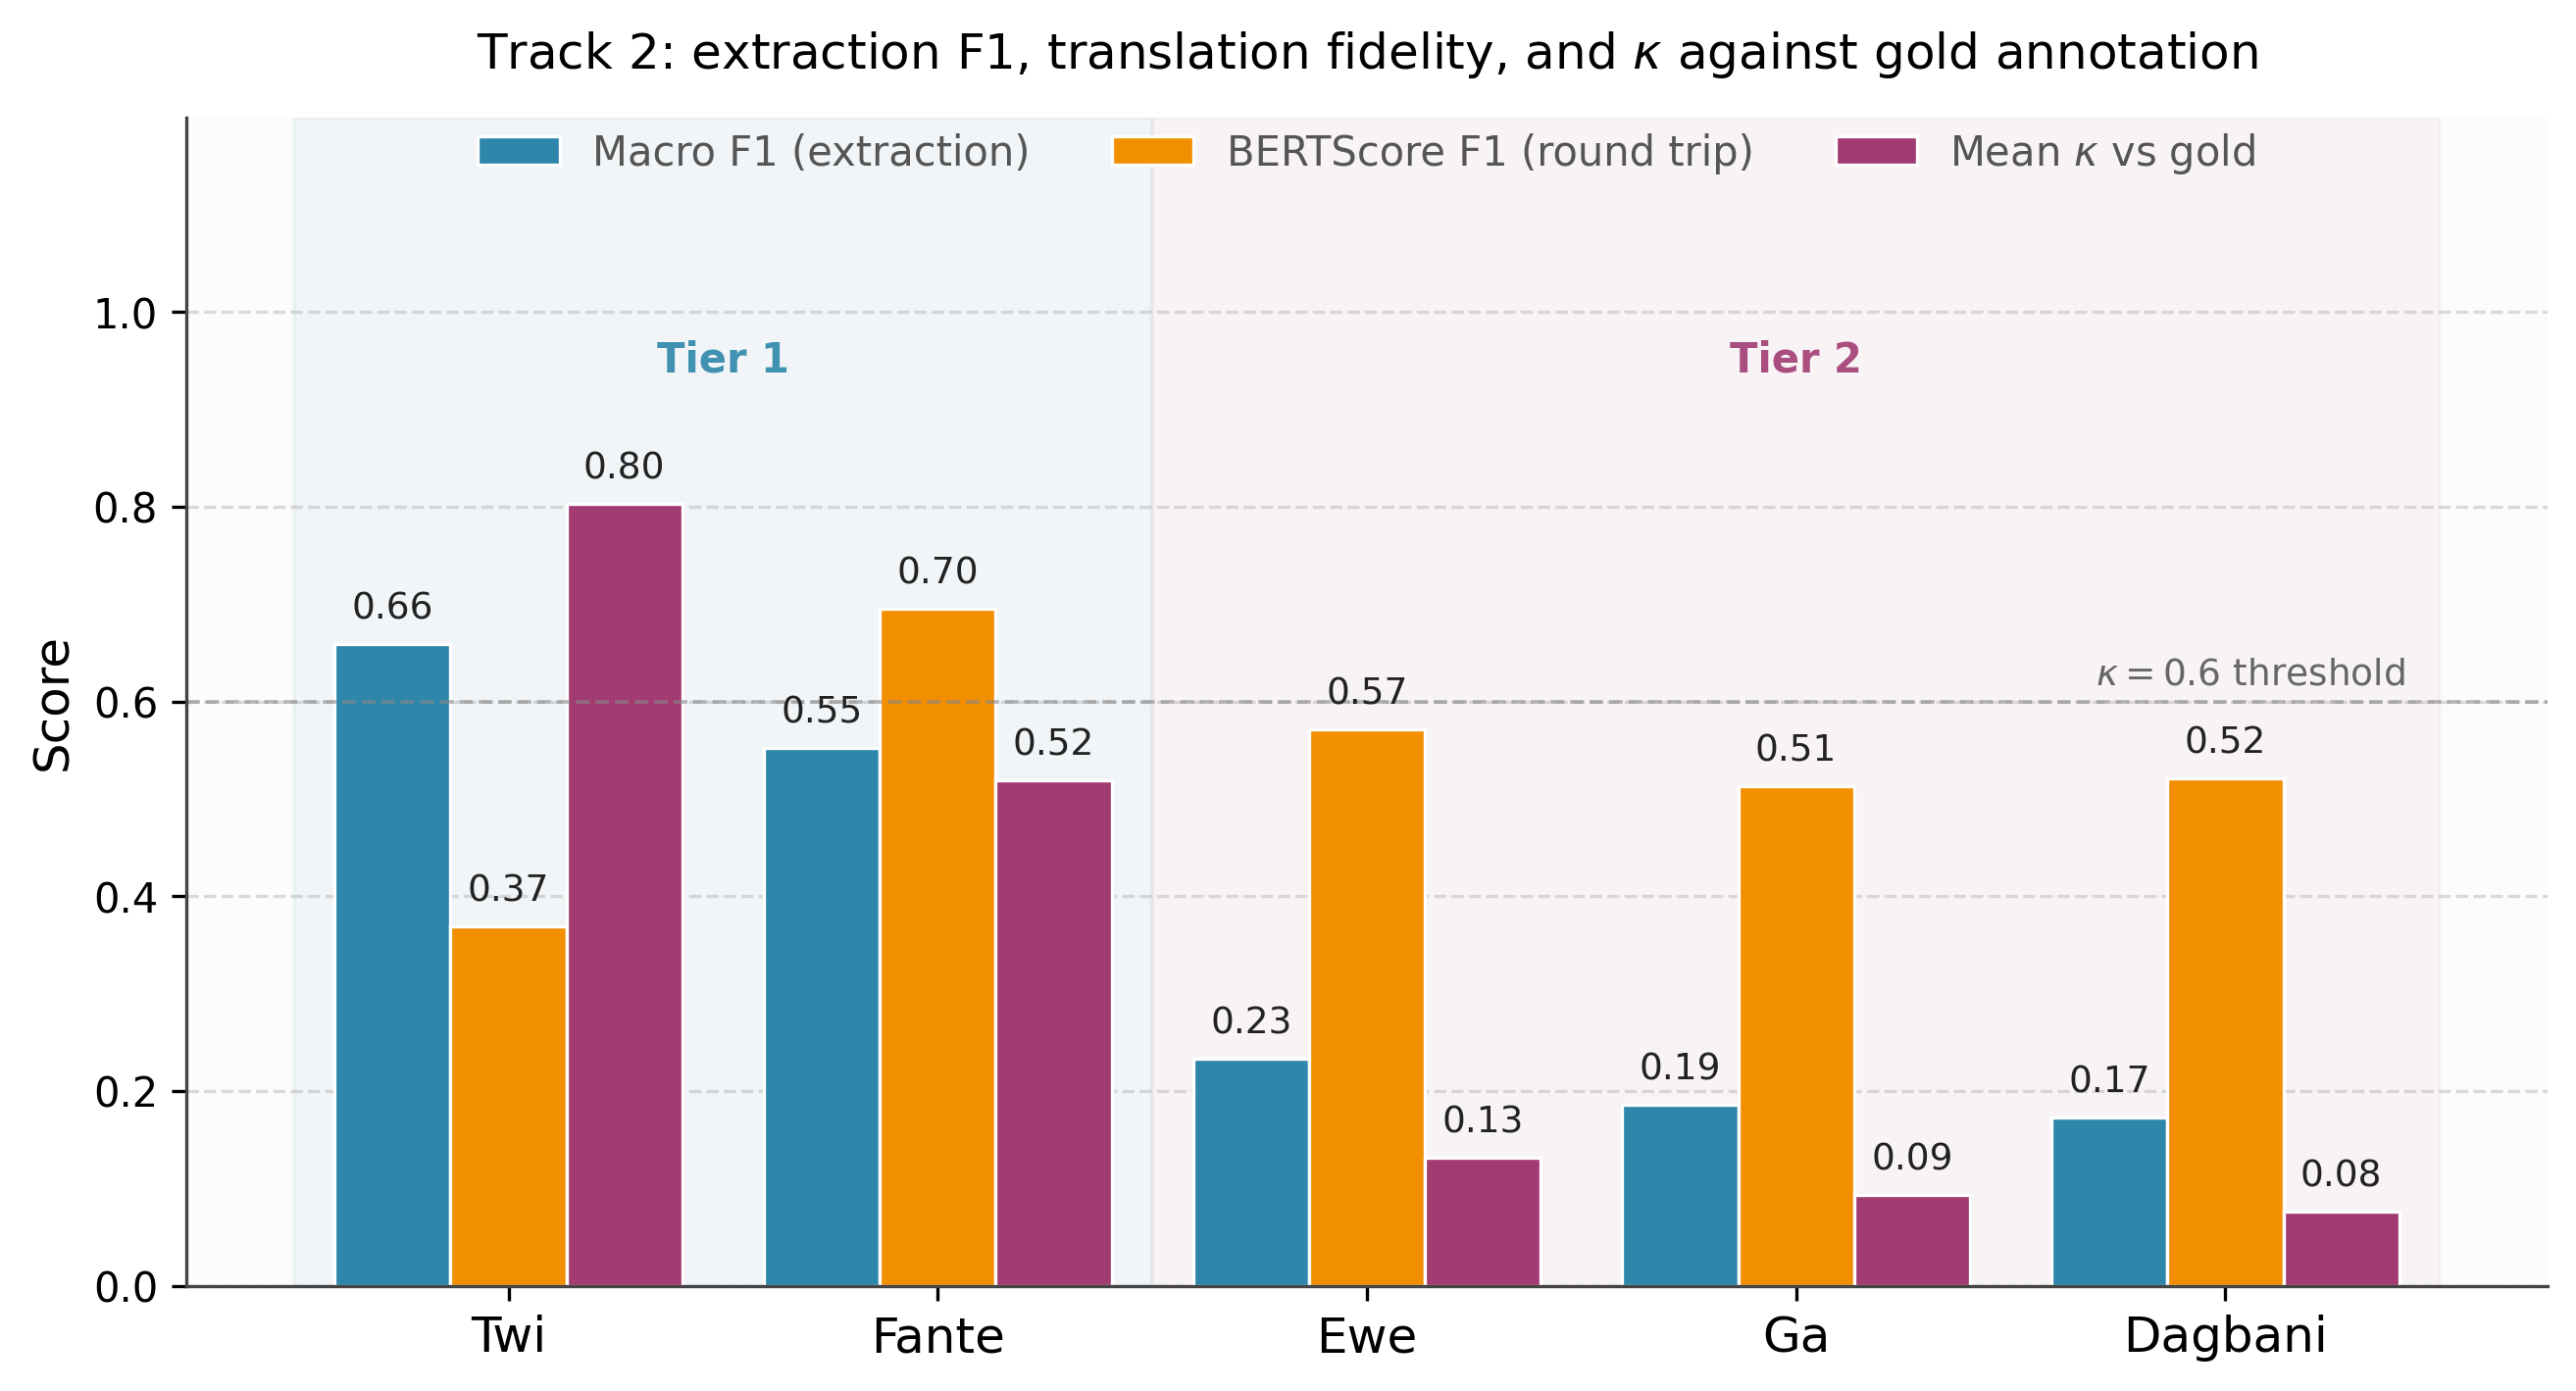
\includegraphics[width=\columnwidth]{figures/f1_by_language.png}
\caption{Track~2 metrics across the five evaluated languages.}
\label{fig:f1_langs}
\end{figure}

\begin{figure}[!t]
\centering
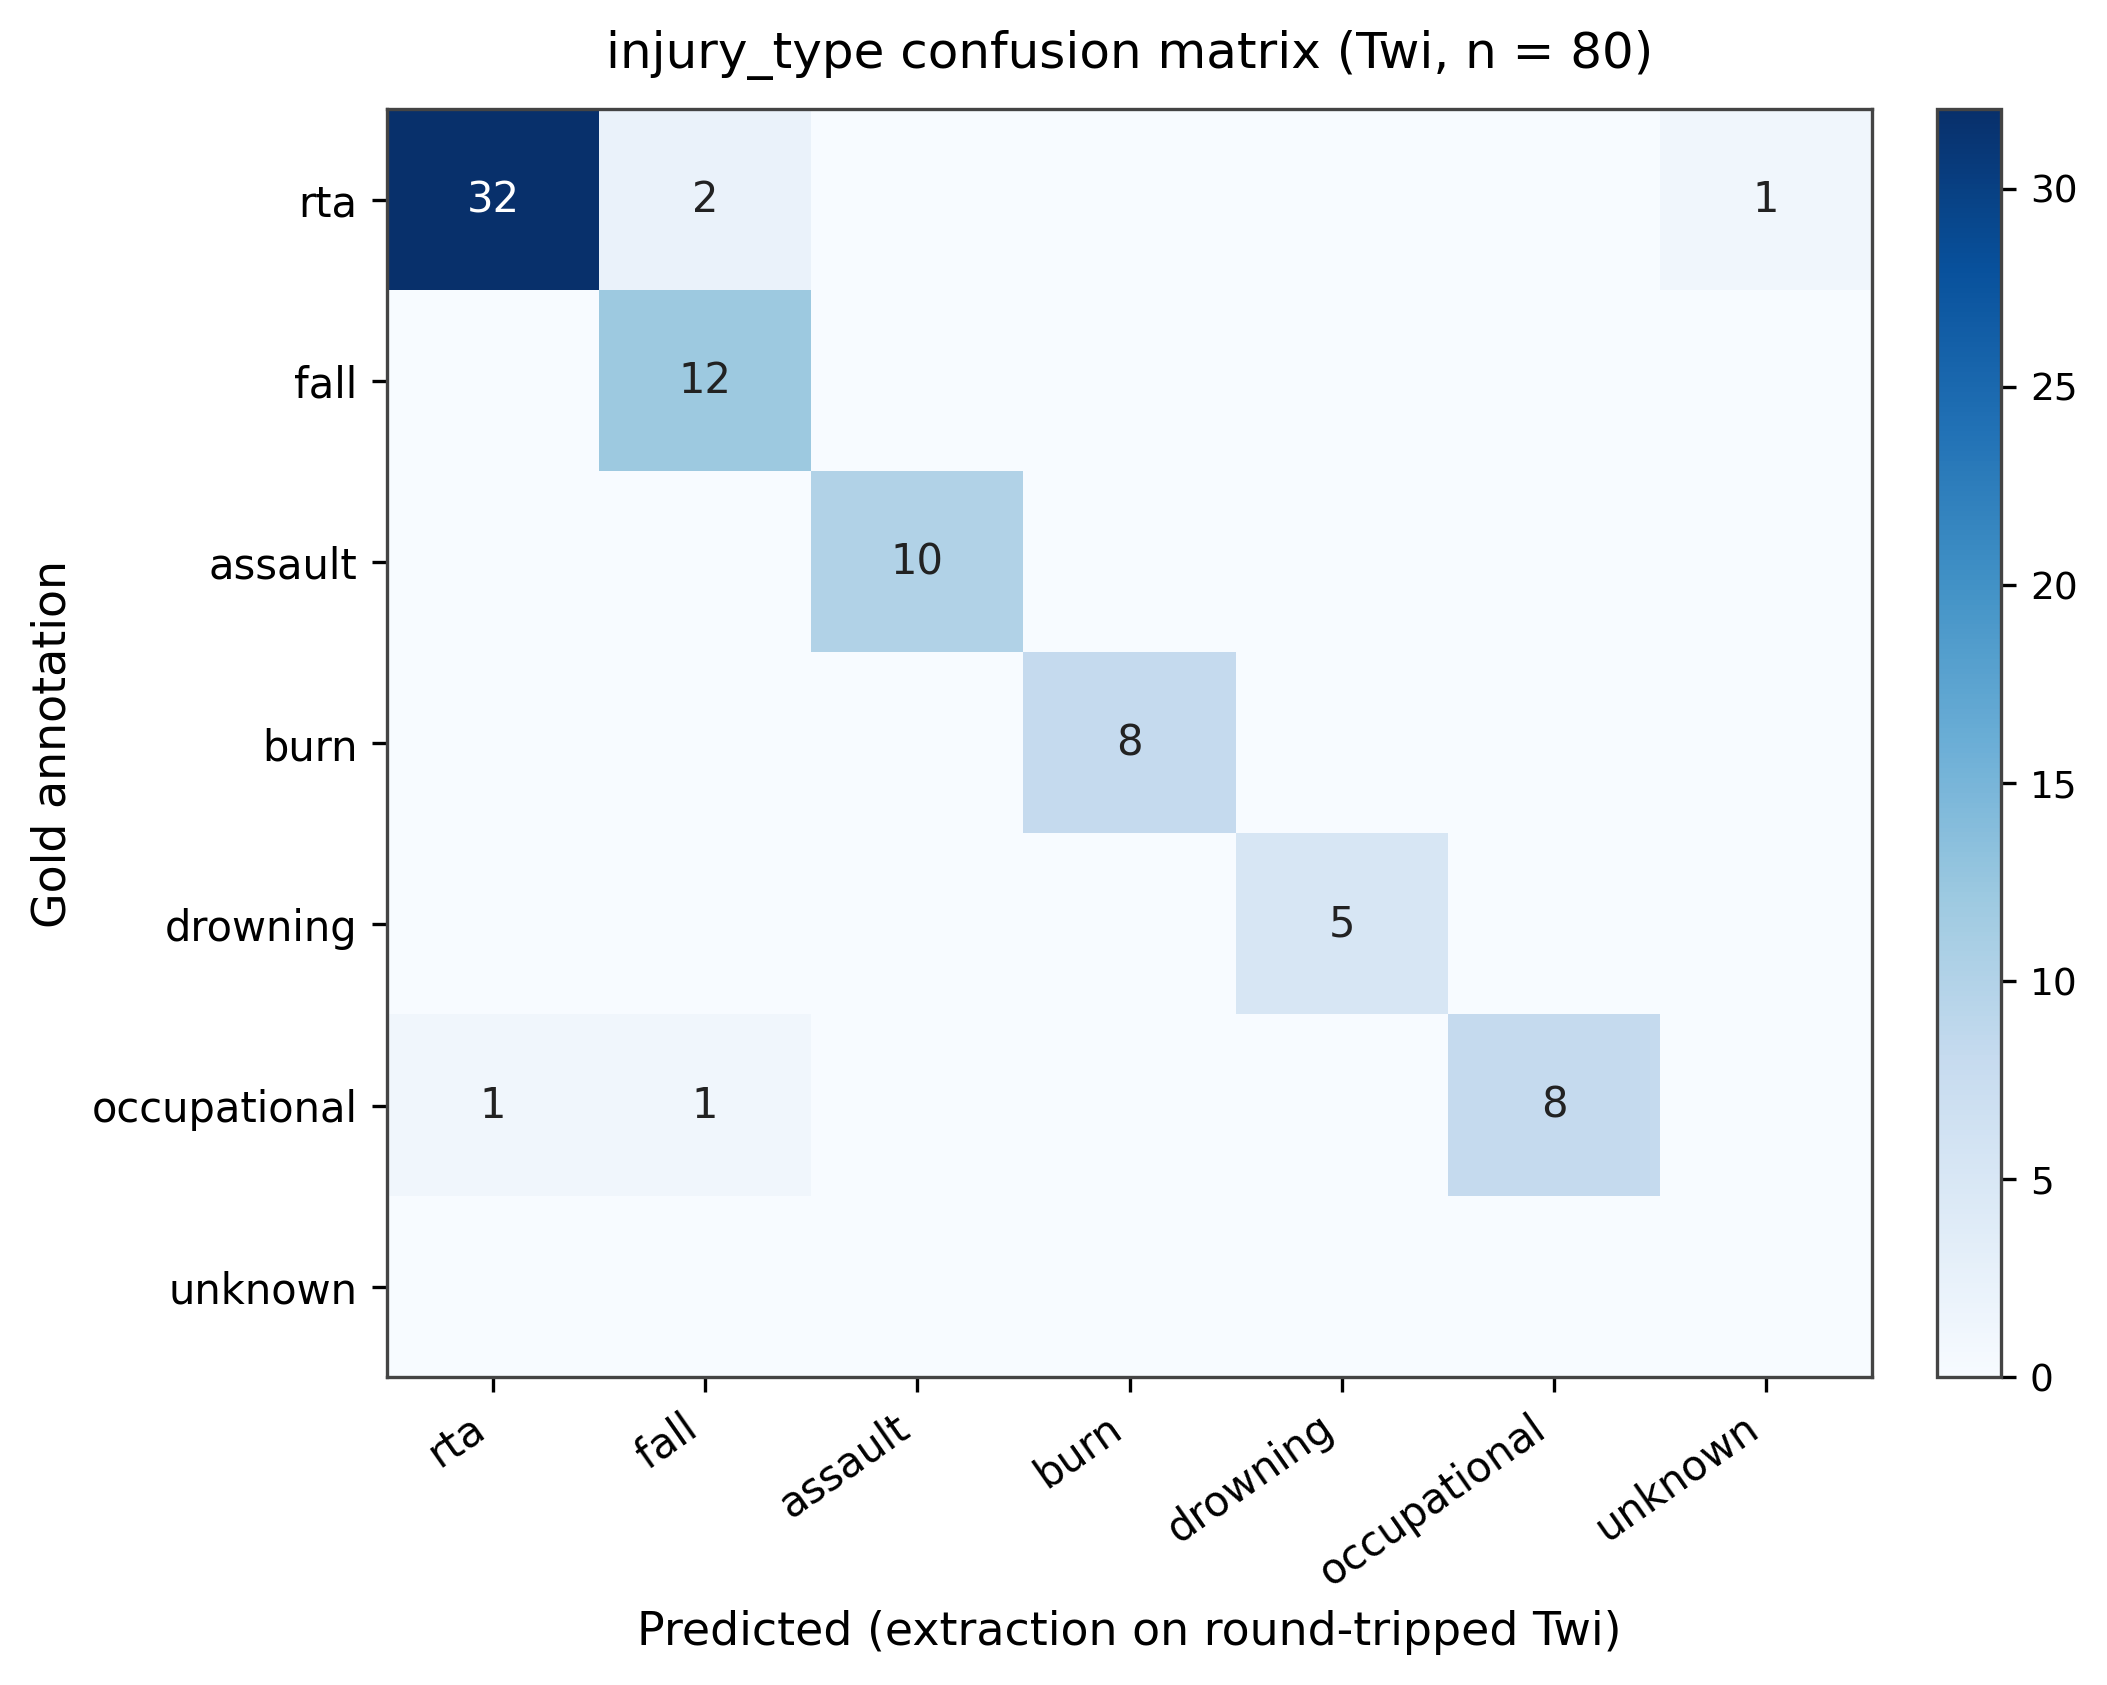
\includegraphics[width=0.92\columnwidth]{figures/confusion_twi_injury.png}
\caption{Track-2 \texttt{injury\_type} confusion matrix for Twi
($n = 80$). Off-diagonal mass concentrates on a single
\textit{rta}$\rightarrow$\textit{fall} confusion class.}
\label{fig:cm_twi}
\end{figure}

\paragraph{Per-class behaviour for \texttt{injury\_type}.}
Figure~\ref{fig:cm_twi} reports the Track-2 confusion matrix for
the \texttt{injury\_type} field on Twi. Diagonal mass exceeds 95\%,
consistent with the per-field $\kappa = 0.92$ reported in
Table~\ref{tab:kappa_gold}. The dominant residual error class is
the substitution of \textit{fall} for \textit{rta}, which is
linguistically explicable: the Twi descriptor for an
\textit{accident-fall} from a vehicle overlaps lexically with the
descriptor for a non-vehicular fall, and the round-trip translation
collapses the distinction in a small number of cases.

\paragraph{Agreement against gold.}
Table~\ref{tab:kappa_gold} reports per-language mean $\kappa$ against
the gold annotation. Following the conventional thresholds of Landis
and Koch~\cite{landis1977}, $\kappa > 0.80$ indicates near-perfect
agreement and $\kappa > 0.60$ indicates substantial agreement. Twi
($\kappa = 0.80$) and Fante ($\kappa = 0.52$) meet the operational
threshold of substantial-or-better agreement on at least one core
field; Ga, Ewe, and Dagbani record $\kappa < 0.13$, near
chance-level agreement.

\begin{table*}[!t]
\caption{Track~2 mean $\kappa$ against gold annotation per language.}
\label{tab:kappa_gold}
\centering
\begin{tabular}{lcccccc}
\toprule
\textbf{Language}
  & \texttt{injury\_type}
  & \texttt{severity}
  & \texttt{body\_region}
  & \texttt{victim\_sex}
  & \texttt{victim\_age\_group}
  & \textbf{Mean $\kappa$} \\
\midrule
Twi     & 0.92 & 0.71 & 0.81 & 0.95 & 0.64 & \textbf{0.80} \\
Fante   & 0.67 & 0.45 & 0.49 & 0.46 & 0.52 & \textbf{0.52} \\
Ewe     & 0.18 & 0.08 & 0.15 & 0.15 & 0.10 & 0.13 \\
Ga      & 0.20 & $-$0.01 & 0.02 & 0.17 & 0.07 & 0.09 \\
Dagbani & 0.10 & 0.00 & 0.05 & 0.11 & 0.11 & 0.08 \\
\bottomrule
\end{tabular}
\end{table*}

\paragraph{Cross-language consistency.}
Table~\ref{tab:kappa} reports Track-3 cross-language $\kappa$ with
Twi as reference. Twi/Fante records mean $\kappa = 0.51$, while
Twi/Ga, Twi/Ewe, and Twi/Dagbani each record mean $\kappa < 0.13$.
The ranking aligns with the Track-2 BERTScore and BLEU ranking,
indicating that the cross-language gap is propagated by translation
fidelity rather than introduced by the extraction stage.

\begin{table*}[!t]
\caption{Track~3 cross-language extraction consistency
(Cohen's $\kappa$ with Twi as reference).}
\label{tab:kappa}
\centering
\begin{tabular}{lccccc}
\toprule
\textbf{Field}
  & \textbf{Twi/Ga}
  & \textbf{Twi/Ewe}
  & \textbf{Twi/Fante}
  & \textbf{Twi/Dagbani}
  & \textbf{Average} \\
\midrule
injury\_type       & 0.19 & 0.16 & 0.65 & 0.10 & 0.28 \\
severity           & 0.08 & 0.05 & 0.43 & 0.00 & 0.14 \\
body\_region       & 0.04 & 0.14 & 0.46 & 0.07 & 0.18 \\
victim\_sex        & 0.16 & 0.11 & 0.47 & 0.11 & 0.21 \\
victim\_age\_group & 0.04 & 0.12 & 0.55 & 0.15 & 0.22 \\
\midrule
\textbf{Average}   & 0.10 & 0.12 & 0.51 & 0.08 & \textbf{0.20} \\
\bottomrule
\end{tabular}
\end{table*}


%% =========================================================
\section{Discussion}
\label{sec:discussion}
%% =========================================================

\subsection{Pipeline Performance}

Twi WER of 51.4\% is consistent with the lexical difficulty of
medical, anatomical, and location-specific vocabulary in a
low-resource language. The injury-type stratification within Twi
spans 5.7~percentage points (47.5\%--53.2\%), with assault narratives
attaining the lowest WER and RTA and fall narratives attaining the
highest. Post-ASR macro-$F_{1}$ of 0.43, against 0.66 on clean
text, isolates the cost of ASR noise at $\Delta F_{1} = 0.23$. The
severity field absorbs the largest reduction
($F_{1} = 0.29$), indicating that severity cues are concentrated in
short lexical items that are particularly sensitive to ASR
substitution.

Fante reproduces the same pattern at a lower baseline. Post-ASR
macro-$F_{1}$ falls from 0.55 to 0.34 ($\Delta F_{1} = 0.21$), in
keeping with the higher baseline WER of 61.0\%. Recovery to
$\kappa = 0.52$ on clean text indicates that the extraction
architecture remains within useful operating range for Fante; the
binding constraint at the language level is ASR accuracy.

Track-2 BERTScore $F_{1}$ varies from 0.369 (Twi) to 0.695 (Fante),
and BLEU from 1.86 to 15.86. The Twi inversion---low surface-form
fidelity, high extraction $F_{1}$ and $\kappa$---is consistent with
agglutinative morphology: round-trip translation produces divergent
surface forms while preserving the predicate-argument structure on
which extraction depends. For Ga, Ewe, and Dagbani, extraction
$F_{1}$ remains in the range 0.17--0.23 and $\kappa$ remains below
0.13, while BERTScore stays in the 0.51--0.57 range. The combination
indicates partial round-trip fidelity that is insufficient to
preserve the categorical content required by extraction.

Track-3 mean $\kappa = 0.20$ across Twi-anchored pairs reproduces
the Tier-1 / Tier-2 split observed in Track~2. Twi/Fante reaches
$\kappa = 0.51$; the remaining Twi-anchored pairs fall below $0.13$.
Because the extraction prompt is invariant across languages, the
cross-language gap propagates the Track-2 translation gap; the
binding constraint for the Tier-2 languages is therefore MT capacity.

\subsection{The Ga ASR Outlier}
\label{sec:ga_outlier}

Ga WER of 80.9\% exceeds the next-highest language by
19.9~percentage points and warrants separate treatment. The most
plausible mechanism is acoustic mismatch between the Khaya TTS
synthesis voice for Ga and the acoustic profile expected by the
Khaya Ga ASR model. For languages with stronger ASR training
coverage, the same TTS$\rightarrow$ASR loop is less affected.
Reported Ga WER is therefore an evaluation-design artefact rather
than an upper bound on Ga ASR performance under natural speech.

\subsection{Clinical Safety}
\label{sec:safety}

The first-aid component introduces a safety dimension that does not
arise in pure data-collection systems. Three constraints are
enforced at the prompt level on every generated response. First,
each response is framed as guidance pending professional care.
Second, every response ends with an instruction to attend the
nearest health facility, regardless of severity. Third, the prompt
forbids diagnostic claims, drug recommendations, and treatment
specifications. The system is not designed to substitute for
emergency dispatch or clinical assessment; its scope is limited to
the pre-facility information bridge.

\subsection{Evaluation Limitations}
\label{sec:limitations}

The TTS$\rightarrow$ASR evaluation loop introduces an acoustic
circularity: TTS-synthesised audio is closer in distribution to the
training data of the same vendor's ASR than natural community speech
is likely to be. Track-1 results should therefore be read as
optimistic lower bounds on real-world WER. The Ga outlier in
Section~\ref{sec:ga_outlier} is one observable consequence of this
circularity.

The two-pass single-annotator gold standard limits annotation
diversity. Inter-pass agreement is reported as the available proxy
for inter-annotator reliability; multi-annotator labelling is
identified as a priority for any subsequent corpus release.

The synthetic corpus is grounded in published Ghanaian
distributions, but does not yet contain real caller utterances.
Generalisation of the reported metrics to natural community speech
is empirically untested, and no causal claim is made about real-world
deployment performance on the basis of Track-1 results alone.

\subsection{Future Work}

Three priorities follow directly from the limitations above.
First, evaluation on natural speech recruited from community health
workers and crash witnesses would replace the synthetic
TTS$\rightarrow$ASR loop with realistic acoustic input. Second, a
controlled community pilot in a Twi- or Fante-speaking area would
validate the geocoding and surveillance logging components under
operational conditions and would also generate the natural-speech
corpus required for the first priority. Third, the deployment
infrastructure---a dedicated shortcode, an integration to DHIMS-2,
and a forwarding protocol to the National Ambulance Service---is a
health-systems engineering task that is outside the scope of the
present pipeline but is the explicit motivation for it.


%% =========================================================
\section{Conclusion}
\label{sec:conclusion}
%% =========================================================

This paper has presented VoiceTrace, a five-stage NLP pipeline that
produces both a spoken first-aid response and a structured geocoded
surveillance record from a single voice call in a Ghanaian language.
The pipeline is constructed entirely from existing in-country
language technology (Khaya ASR, MT, and TTS) together with zero-shot
LLM extraction. An epidemiologically grounded synthetic corpus of
126 narratives has been released as a reproducible benchmark, and a
three-track evaluation has separated ASR error, translation
fidelity, and extraction consistency.

Empirically, technical feasibility is demonstrated for Twi
(macro-$F_{1} = 0.66$ on clean text, $0.43$ post-ASR;
$\kappa = 0.80$ against gold) and partial feasibility for Fante
(macro-$F_{1} = 0.55$; $\kappa = 0.52$). For Ga, Ewe, and Dagbani,
the binding constraint is MT capacity rather than the extraction
architecture; the work establishes the first quantitative baseline
for these three languages in this task.

Three subsequent decisions, none of them technical, are required
before community deployment: a dedicated shortcode assigned by the
National Communications Authority; an integration between the
VoiceTrace surveillance log and the Ghana Health Service DHIMS-2;
and a forwarding protocol between VoiceTrace and the National
Ambulance Service dispatch network. The authors invite collaboration
with the National Ambulance Service, the Ghana Health Service, and
the GhanaNLP consortium toward a community pilot.

All code and the synthetic corpus will be released under an open
licence to support replication and independent audit
(Section~\ref{sec:repro}).


%% =========================================================
\section*{Ethics Statement}
%% =========================================================

The evaluation corpus is synthetic and is generated from published
aggregate injury statistics; no personal health information, no
identifiable individual data, and no recordings of real callers were
collected, processed, or stored. The work involves no human subjects
in the experimental sense, and no institutional review board approval
was therefore required for the experiments reported here. The
first-aid response component is constrained at the prompt level to
prohibit diagnostic claims, drug recommendations, and treatment
specifications, and every response directs the caller to the nearest
health facility. Subsequent deployment with real caller data will
require institutional review, informed consent procedures suited to
spoken interaction, secure handling of voice and location data, and
explicit governance over how surveillance records are accessed by
health authorities.


%% =========================================================
\section*{Declaration on the Use of Generative AI}
%% =========================================================

The authors disclose the use of generative AI in this work. Claude
(\texttt{claude-sonnet-4-6})~\cite{anthropic2024} is a system
component: it performs structured extraction and first-aid generation
in Stage~3 of the pipeline (Section~\ref{sec:arch}) and was used to
author the 126 synthetic narratives that constitute the evaluation
corpus (Section~\ref{sec:data}). Outputs were inspected by the
authors and either accepted, edited, or discarded. During manuscript
preparation, generative AI was additionally used in a limited
assistive capacity for copy-editing and prose tightening. All
scientific claims, experimental designs, statistical analyses, and
interpretations were formulated, executed, and verified by the
authors, who accept full responsibility for the content of this
paper.


%% =========================================================
\section*{Reproducibility and Data Availability}
\label{sec:repro}
%% =========================================================

The 126-narrative synthetic corpus, the gold annotations, the
evaluation scripts, and the VoiceTrace source code will be released
under an open licence on acceptance. The release will include the
language-specific TTS audio, the ASR transcripts, and the prompts
used for narrative generation and extraction, sufficient to
reproduce the results in Section~\ref{sec:eval} end to end. External
dependencies (Khaya API, Anthropic Claude API, Nominatim,
OpenStreetMap) are reachable through their public endpoints. Random
seeds, model versions (\texttt{claude-sonnet-4-6}; Khaya ASR~v3 and
TTS~v2), and library versions are recorded in the released
configuration files.


%% =========================================================
\section*{Author Contributions}
%% =========================================================

\textbf{Y.~O.~Adjei} conceived the study, designed and implemented
the pipeline, designed the evaluation framework, conducted the
experiments, and drafted the manuscript.
\textbf{D.~Opoku} contributed to dataset construction, gold
annotation, and statistical analysis.
\textbf{K.~A.~Owusu} contributed to system architecture, geocoding,
and the surveillance-logging pathway.
\textbf{B.~T.~Partey} provided technical guidance on injury
surveillance system design, data architecture, and analytical
methodology, and supervised the manuscript.
All authors reviewed and approved the final manuscript.


%% =========================================================
\section*{Funding and Competing Interests}
%% =========================================================

This work received no external funding. The authors declare no
competing financial or non-financial interests. API access to
Anthropic Claude was provided at no cost; the programme had no role
in the study design, the analyses, or the decision to publish.


%% =========================================================
\section*{Acknowledgements}
%% =========================================================

The authors thank the GhanaNLP team for access to the Khaya API, and
the Kwame Nkrumah University of Science and Technology Centre for
Injury Prevention and Research for hosting this conference.


%% =========================================================
%% REFERENCES
%% =========================================================
\sloppy
\begin{thebibliography}{99}

\bibitem{graphic2026_nrsa}
T.~Ngenbe,
``Road crashes killed 2{,}949 in Ghana in 2025, the highest in 35
years,''
\textit{Graphic Online}, Daily Graphic, Accra, Ghana, Jan. 2026.
[Online]. Available:
\url{https://www.graphic.com.gh/news/general-news/road-crashes-killed-2-949-in-ghana-in-2025-the-highest-in-35-years-road-safety-authority.html}

\bibitem{boateng2019}
S.~Boateng, A.~Acheampong, B.~Appiah, and E.~Hagan,
``Pattern of injuries seen at the Accident and Emergency Centre of
the Korle-Bu Teaching Hospital, Accra, Ghana,''
\textit{Ghana Med. J.}, vol.~53, no.~1, pp.~46--52, Mar. 2019,
doi:\,10.4314/gmj.v53i1.7.

\bibitem{opoku2025}
D.~A.~Opoku, E.~Forson, and A.~Mensah,
``Burden and pattern of injuries in Ghana: a systematic review and
meta-analysis of hospital-based studies,''
\textit{BMC Public Health}, vol.~25, 2025.

\bibitem{mesic2024}
A.~Mesic, K.~A.~Doyle, A.~Gyamfi, and A.~Razzak,
``Spatial analysis of road traffic crash hotspots in Greater Accra,
Ghana,''
\textit{Injury Epidemiol.}, vol.~11, no.~1, p.~32, 2024,
doi:\,10.1186/s40621-024-00517-5.

\bibitem{who_ghe}
World Health Organization,
``Global Health Estimates 2024: Deaths by Cause, Age, Sex, by
Country and by Region, 2000--2021,''
WHO, Geneva, 2024.
[Online]. Available:
\url{https://www.who.int/data/global-health-estimates}

\bibitem{ihme_gbd}
Institute for Health Metrics and Evaluation,
``Global Burden of Disease Study 2021: Ghana Results,''
IHME, Seattle, WA, 2024.
[Online]. Available:
\url{https://vizhub.healthdata.org/gbd-results/}

\bibitem{dhs2022}
Ghana Statistical Service, Ghana Health Service, and ICF,
``Ghana Demographic and Health Survey 2022,''
GSS, GHS, and ICF, Accra and Rockville, MD, 2024.
[Online]. Available:
\url{https://dhsprogram.com/pubs/pdf/FR378/FR378.pdf}

\bibitem{dhs2008}
Ghana Statistical Service, Ghana Health Service, and Macro
International,
``Ghana Demographic and Health Survey 2008,''
GSS, GHS, and Macro International, Accra and Calverton, MD, 2009.
[Online]. Available:
\url{https://dhsprogram.com/pubs/pdf/FR221/FR221.pdf}

\bibitem{khaya}
GhanaNLP,
``Khaya API: ASR, MT, and TTS for Ghanaian languages,''
2024. [Online]. Available: \url{https://ghananlp.org}.
Accessed Apr. 2026.

\bibitem{radford2023}
A.~Radford, J.~W.~Kim, T.~Xu, G.~Brockman, C.~McLeavey, and
I.~Sutskever,
``Robust speech recognition via large-scale weak supervision,''
in \textit{Proc. 40th Int. Conf. Mach. Learn. (ICML)},
Honolulu, HI, USA, Jul. 2023, pp.~28492--28518.

\bibitem{vallmuur2015}
K.~Vallmuur,
``Machine learning advances in analysing routinely collected injury
surveillance data: opportunities and challenges,''
\textit{Injury Epidemiol.}, vol.~2, no.~1, p.~20, Dec. 2015,
doi:\,10.1186/s40621-015-0056-1.

\bibitem{morris2004}
A.~Morris, V.~Maier, and P.~Green,
``From WER and RIL to MER and WIL: improved evaluation measures for
connected speech recognition,''
in \textit{Proc. Interspeech}, Jeju, Korea, 2004, pp.~2765--2768.

\bibitem{omiye2025}
J.~A.~Omiye, H.~Gui, J.~S.~Rezaei, R.~Zou, and R.~Daneshjou,
``Large language models in medicine: the potentials and pitfalls,''
\textit{Nat. Med.}, vol.~30, pp.~1113--1117, 2024,
doi:\,10.1038/s41591-024-02958-5.

\bibitem{lorenzoni2024}
V.~Lorenzoni, G.~Turchetti, and G.~Navigli,
``Evaluating large language models for clinical information
extraction and coding,''
\textit{JAMIA Open}, vol.~7, no.~2, 2024,
doi:\,10.1093/jamiaopen/ooae049.

\bibitem{nyamawe2026}
A.~S.~Nyamawe and N.~Shao,
``Leveraging large language models for low-resource African language
NLP: a synthetic data approach,''
\textit{arXiv preprint}, 2026.

\bibitem{zhang2019bertscore}
T.~Zhang, V.~Kishore, F.~Wu, K.~Q.~Weinberger, and Y.~Artzi,
``BERTScore: Evaluating text generation with BERT,''
in \textit{Proc. 8th Int. Conf. Learn. Representations (ICLR)},
Addis Ababa, Ethiopia, 2020.
[Online]. Available:
\url{https://openreview.net/forum?id=SkeHuCVFDr}

\bibitem{anthropic2024}
Anthropic,
``Claude model documentation: Sonnet, Opus, Haiku,''
Anthropic, San Francisco, CA, USA, 2024--2026.
[Online]. Available: \url{https://docs.anthropic.com/en/docs/about-claude/models}.
Accessed Apr. 2026.

\bibitem{ghc2021}
Ghana Statistical Service,
``Ghana 2021 Population and Housing Census: General Report,''
GSS, Accra, Ghana, 2023.
[Online]. Available:
\url{https://statsghana.gov.gh/gssmain/fileUpload/pressrelease/2021PHCGeneralReport.pdf}

\bibitem{landis1977}
J.~R.~Landis and G.~G.~Koch,
``The measurement of observer agreement for categorical data,''
\textit{Biometrics}, vol.~33, no.~1, pp.~159--174, Mar. 1977,
doi:\,10.2307/2529310.

\end{thebibliography}

\end{document}
